\definecolor{singleShotColor}{RGB}{196,106,28}
\definecolor{pipelineColor}{RGB}{44,138,100}
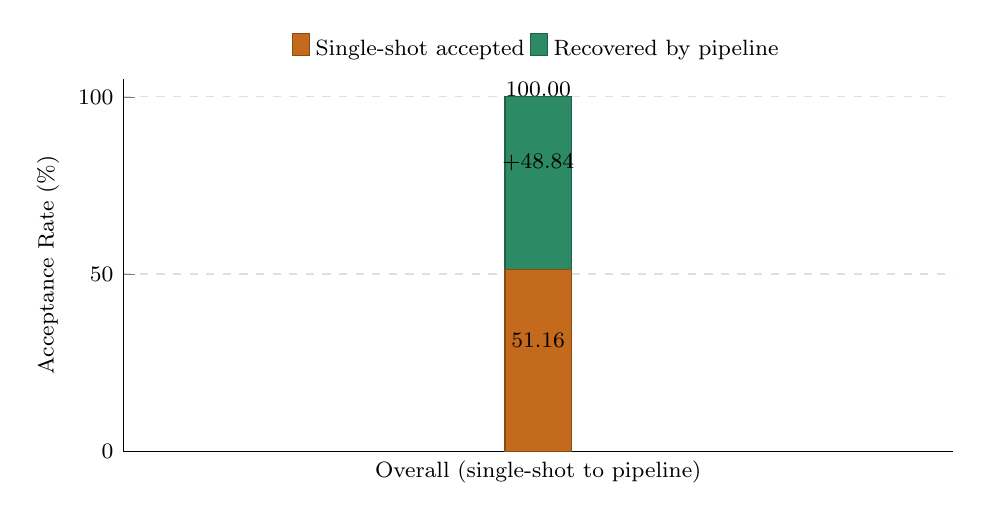
\begin{tikzpicture}
\begin{axis}[
    ybar stacked,
    bar width=24pt,
    width=\columnwidth,
    height=0.52\columnwidth,
    ymin=0,
    ymax=105,
    ylabel={Acceptance Rate (\%)},
    symbolic x coords={Overall},
    xtick=data,
    xticklabels={Overall (single-shot to pipeline)},
    x tick label style={font=\footnotesize, align=center},
    axis lines*=left,
    ymajorgrids=true,
    grid style={dashed,gray!25},
    tick label style={font=\footnotesize},
    label style={font=\footnotesize},
    legend style={
        draw=none,
        font=\footnotesize,
        at={(0.5,1.02)},
        anchor=south,
        legend columns=2
    },
]
\addplot+[
    fill=singleShotColor,
    draw=singleShotColor!70!black,
    nodes near coords,
    every node near coord/.append style={font=\footnotesize, text=black, anchor=south, yshift=1pt},
] coordinates {(Overall,51.16)};

\addplot+[
    fill=pipelineColor,
    draw=pipelineColor!70!black,
    nodes near coords,
    every node near coord/.append style={font=\footnotesize, text=black, anchor=south, yshift=1pt},
    point meta=explicit symbolic,
    nodes near coords={+\pgfmathprintnumber[fixed,precision=2]{\pgfplotspointmeta}},
] coordinates {(Overall,48.84) [48.84]};

% Top label (pipeline total)
\node[font=\footnotesize] at (axis cs:Overall,102.0) {100.00};

\legend{Single-shot accepted,Recovered by pipeline}
\end{axis}
\end{tikzpicture}
